\documentclass{article}
\usepackage{graphicx} % Required for inserting images
\usepackage[bottom=2cm,top=2cm,right=1.5cm,left=1cm,binding=1cm]{geometry}
\usepackage{mathtools}
\usepackage{cancel}
\usepackage{pgfplots}
\pgfplotsset{compat = newest}
\usetikzlibrary{arrows.meta}
\usepackage{tikz}
\title{Entregables electrodinámica clásica}
\author{Álvaro Méndez Rodriguez de Tembleque}
\date{\today}

\begin{document}

\maketitle

\section{Entregable 1}
\subsection{Se detectan luz y neutrinos muy energéticos/ ultrarrelativisticos después de un evento cósmico. Los neutrinos llegan con un retraso corto de entre 1·dt y 4·dt después de la luz. Asumiendo que todos salieron al mismo tiempo en la explosión, ¿Qué relación hay entre las energías de los primeros (1·dt) y últimos (4·dt) neutrinos?}
Para realizar este problema vamos a asumir que nos encontramos en unn sistema $S$, es decir, no nos encontramos sobre ninguna de las partículas y además supondremos que todas recorren la misma trayectoría $x$, de esta forma tenemos que los fotones recorren una distancia $x$ en un tiempo $t$, los primeros neutrinos ($\nu_{1}$) en un tiempo $t_{1}=t+dt$ y los segundos neutrinos ($\nu_{2}$) en un tiempo $t_{2}=t+4dt$. 

De esta forma tenemos que las trayectorias de las partículas son:
\[x=ct \qquad x=v_{1}(t+dt) \qquad x=v_{2}(t+4dt)\]

De esta forma podemos obtener $dt$ para cada una de las partículas como:
\begin{itemize}
  \item Primeros neutrinos $\nu_{1}$
  
  Despejando 
  
  \[\left.\begin{aligned}
    t=\frac{x}{c}\\
    dt=\frac{x}{v_{1}}-t
    \end{aligned}\right\}dt=x(\frac{1}{v_{1}}-\frac{1}{c})=\frac{x}{c}(\frac{1}{\beta_{1}}-1)\]
  Dado que los neutrinos son partículas muy ligeras y rápidas, podemos asumir que nos encontramos en el caso ultrarelativista en donde podemos aproximar por serie de Taylor 
  \[\frac{1}{\beta}\sim1+\frac{1}{2\gamma^{2}}\]
  Entonces podemos definir $dt$ como:
  \[dt=\frac{x}{2c\gamma_{1}^{2}}\]
  \item Segundos neutrinos $\nu_{2}$
  
  De forma completamente idéntica al caso anterior podemos despejar $dt$ como 
  \[dt=\frac{1}{4}(\frac{x}{v_{2}}-t)= \frac{x}{4c}(\frac{1}{\beta_{2}}-1)\]
  Por serie de taylor llegamos a 
  \[dt=\frac{x}{8c\gamma_{2}^{2}}\]
\end{itemize}

Una vez calculados los $dt$ de cada grupo de neutrinos podemos relacionarlos entre si de la forma
\[\left.\begin{aligned}
  dt=\frac{x}{2c\gamma_{1}^{2}}\\
  dt=\frac{x}{8c\gamma_{2}^{2}}
\end{aligned}\right\}\frac{dt}{dt}=\frac{\frac{x}{2c\gamma_{1}^{2}}}{\frac{x}{8c\gamma_{2}^{2}}}\xrightarrow{\text{Despejando los }\gamma}\frac{\gamma_{1}}{\gamma_{2}}=2\] 

Una vez obtenido la relación entre los coeficientes $\gamma$ entre ambas especies de neutrinos, comparamos la relación que hay entre sus energías, las cuales, dado el caso en el que nos encontramos, tendran la forma 
\[E_{i}=\gamma_{i}mc^{2}\]

Entonces 
\[\frac{E_{1}}{E_{2}}=\frac{\gamma_{1}mc^{2}}{\gamma_{2}mc^{2}}=\frac{\gamma_{1}}{\gamma_{2}}=2\]
\subsection{Dos ondas planas electromagnéticas se propagan en la misma dirección y sentido, con la misma frecuencia y están circularmente polarizadas en el mismo sentido a la derecha, pero con intensidades promediadas de I y 4·I, respectivamente. Considerar dos casos: 1. están en fase; 2. hay un desfase de $\frac{\pi}{2}$.
Calcular la intensidad promediada e indicar la polarización de la onda superpuesta (para ambos casos).}

Las ondas descritas por el enunciado son ondas RHCP, asumiendo que se propagan en el eje $\hat{z}$ y con la misma frecuencia, que en fasores se pueden escribir como:
\[\vec{E}=E_{0}(\hat{x}-i\hat{y}) \frac{1}{\sqrt{2}}e^{i\omega(t-\frac{z}{c})}\]

La intensidad de una onda $I$ se define como $I=\vec{E}^{2}$, obtenemos la intensidad de la primera onda de la siguiente forma, con $\vec{E_{1}}=\vec{E}$

\[I_{1}\equiv I=\vec{E_{1}}^{2}=\frac{E_{0}^{2}}{2}(\underbrace{\hat{x}\cdot \hat{x}}_{1}+\overbrace{i \hat{x}\cdot \hat{y}- i \hat{x}\cdot \hat{y}}^{0}+\underbrace{\hat{y}\cdot \hat{y}}_{1})=E_{0}^{2}\]

Para encontrar la relación que se nos da en el enunciado definimos la onda $\vec{E_{2}}$ como proporcional a la onda $\vec{E_{1}}$, de forma que $\vec{E_{2}}=a \vec{E_{1}}$ y obtenemos su intensidad como:

\[I_{2}= \vec{E_{2}}^{2}=a^{2} \vec{E_{1}}^{2}= a^{2}I\]

Por el enunciado sabemos que $a$ tiene que ser igual a 2 para obtener la relacion $I_{2}=4I$. 

Ahora calculamos las intensidades de la superposición de ambas ondas, tanto en fase como en desfase:

\begin{itemize}
  \item Ondas en fase 
  
  Sumaos las dos ondas ya que inicialmente las hemos considerado en fase:

  \[\vec{E_{f}}=\vec{E_{1}}+\vec{E_{2}}=\frac{E_{0}}{\sqrt{2}}\left[(\hat{x}-i \hat{y})+2(\hat{x}-i \hat{y})\right]e^{i\omega(t-\frac{z}{c})}\]
  \[~~=\frac{3E_{0}}{\sqrt{2}}(\hat{x}-i \hat{y})e^{i\omega(t-\frac{z}{c})}\]
  \[=3\vec{E_{1}}\]

  Como podemos observar la onda superpuesta tiene la misma polarización que la onda inicial $\vec{E}$

  Ahora calculamos $I_{fase}=\vec{E_{f}}^{2}$, que nos queda como 

  \[ I_{f}=9 \vec{E_{1}}^{2}=9I\] 
  \item Ondas desfasadas $\frac{\pi}{2}$
  
  Para tener en cuenta el desfase vamos a contruir una onda como $\vec{E_{2}}$ que este desfasada que llamaremos $\vec{E'_{2}}$ y procedemos de forma análoga a como lo hicimos para la onda en fase. 

  Pero primero vamos a definir esta nueva onda desfasada, para ello añadimos un desfase $\phi=\frac{\pi}{2}$ a la onda, teniendo entonces 
  \[\vec{E'_{2}}=2E_{0}(\hat{x}-i\hat{y}) \frac{1}{\sqrt{2}}e^{i\omega(t-\frac{z}{c}+\frac{\phi}{\omega})}\]

  \[~~=2E_{0}(\hat{x}-i\hat{y}) \frac{1}{\sqrt{2}}e^{i\omega(t-\frac{z}{c})}e^{i\phi}\]

  En este caso, como $e^{i \frac{\pi}{2}}=\cancelto{0}{\cos(\frac{\pi}{2})}+i\cancelto{1}{\sin(\frac{\pi}{2})}=i$, obtenemos entonces que $\vec{E'_{2}}=i \vec{E_{2}}= i 2 \vec{E_{1}}$. Entonces la superposición de estas dos ondas es:
  \[\vec{E_{df}}=\vec{E_{1}}+\vec{E'_{2}}= (1+2i) \vec{E_{1}}\]

  Como podemos ver, en este caso la onda resultante queda tambien proporcional a $\vec{E}$ y por lo tanto con la misma polarización.

  Y la intensidad en el desfase queda como:
  \[I_{df}= \vec{E_{df}}^{2}=(1+2i)^{2}\vec{E_{1}}^{2}=5I\]

  
\end{itemize}
\subsection{Un mesón $B^{*}$ de masa $m^{*}=5325 MeV/c^{2}$ decae en un fotón y un mesón $B$ de masa m. La diferencia entre las masas de los dos mesones es $m^{*}-m=45 MeV/c^{2}$. Calcular la energía del fotón
a.) en el sistema de referencia en el que $B^{*}$ está en reposo,
b.) en el sistema de referencia en el que $B$ está en reposo.}

\[B^{*}\longrightarrow B+\gamma\]
\begin{itemize}
  \item Sistema de referencia en el que $B^{*}$ está en reposo
  
  En este sistema de referencia tenemos que $v_{B^{*}}=0$, podemos usar la conservación del cuadrimomento para obtener la velocidad del mesón $B$

  \[P^{\mu}_{B^{*}}=P^{\mu}_{B}+P^{\mu}_{\gamma}\Rightarrow \begin{pmatrix}
      \frac{E_{B^{*}}}{c} \\
      \vec{p}_{B^{*}}
  \end{pmatrix}=\begin{pmatrix}
      \frac{E_{B}}{c} \\
      \vec{p}_{B}
  \end{pmatrix}+\begin{pmatrix}
    \frac{E_{\gamma}}{c}\\
      \vec{p}_{\gamma}
\end{pmatrix}\]

Sabemos que $\vec{p}_{B^{*}}=0$, que la energía de las partículas tiene la forma $E=\sqrt{p^{2}c^{2}+(mc^{2})^{2}}$ podemos obtener 2 sistemas de ecuaciones separando el cuadrimomento en componetntes de energía y momento lineal:

\[m^{*}c^{2}=\sqrt{p_{B}^{2}c^{2}+(mc^{2})^{2}}+ E_{\gamma}\]
y 
\[0=\vec{p}_{B}+\vec{p}_{\gamma}\]

Sabemos que el momento de un fotón es $\vec{p}_{\gamma}= \frac{E_{\gamma}}{c}$ y que el momento de una partícula en movimiento es $\vec{p}_{B}=\gamma m v$, por lo que la energía del fotón queda \footnote{Asumiendo que se mueven en la misma dirección pero sentido opuesto}
\[E_{\gamma}= \gamma mvc\]
y entonces volviendo a la relación de conservación de las energías tenemos 
\[m^{*}c^{2}=\sqrt{(\gamma mv)^{2}c^{2}+(mc^{2})^{2}}+\gamma mvc\]
\[m^{*}c^{2}=mc(\sqrt{(\gamma v)^{2}+c^{2}}+\gamma v)\]

\[m^{*}c=m(\sqrt{(\gamma v)^{2}+c^{2}}+\gamma v )\]
\[\frac{m^{*}c}{m}=\sqrt{(\gamma v)^{2}+c^{2}}+\gamma v \]
Despejando $\gamma v$ obtenemos que  

\[\gamma v= -c\frac{m^{2}-{m^{*}}^{2}}{2mm^{*}}\]

Sustituyendo en la energía del fotón obtenemos que 

\[E_{\gamma}= -c^{2}\frac{m^{2}-{m^{*}}^{2}}{2m^{*}}=44,81~\left[ MeV\right]\]


  \item Sistema de referencia en el que $B$ está en reposo
  
  En este sistema de referencia tenemos que $v_{B}=0$, podemos usar la conservación del cuadrimomento para obtener la velocidad del mesón $B^{*}$
  
  Utilizando el mismo sistema de ecuación del apartado anterior con la nueva condición obtenemos 
  \[P^{\mu}_{B^{*}}=P^{\mu}_{B}+P^{\mu}_{\gamma}\Rightarrow \begin{pmatrix}
      \frac{E_{B^{*}}}{c} \\
      \vec{p}_{B^{*}}
  \end{pmatrix}=\begin{pmatrix}
      \frac{E_{B}}{c} \\
      \vec{0}
  \end{pmatrix}+\begin{pmatrix}
    \frac{E_{\gamma}}{c}\\
      \vec{p}_{\gamma}
\end{pmatrix}\]

Entonces obtenemos de forma directa que $E_{\gamma}=p_{B^{*}}c=\gamma m^{*}v^{*}c$. 

Ahora de igual manera que en el caso anterior vamos con las energías que nos quedan como 
\[\sqrt{p_{B^{*}}^{2}c^{2}+(m^{*}c^{2})^{2}}=mc^{2}+ E_{\gamma}\]
\[\sqrt{(\gamma m^{*}v^{*})^{2}c^{2}+(m^{*}c^{2})^{2}}=mc^{2}+ \gamma m^{*}v^{*}c\]
\[\sqrt{(\gamma v^{*})^{2}+c^{2}}-\gamma v^{*}=\frac{m}{m^{*}}c\]

Despejando $\gamma v^{*}$ obtenemos 

\[\gamma v= c\frac{{m^{*}}^{2}-m^{2}}{2mm^{*}}\]

Sustituyendo en la energía del fotón obtenemos que 

\[E_{\gamma}= -c^{2}\frac{{m^{*}}^{2}-m^{2}}{2m}=45,192~\left[ MeV\right]\]

\end{itemize}

\newpage

\section{Entregable 2}

\subsection{Describir cualitativamente el movimiento de un electrón, en un campo magnético inhomogéneo que está principalmente dirigido en la dirección $+\hat{x}$, en concreto: 
\[
\vec{B} = B_0 \left[\left( 1 + \frac{x^2}{d^2} \right) \hat{x} - \frac{2xy}{d^2} \hat{y}\right]
\]
El campo está descrito así para tener divergencia 0, pero este principalmente dirigido en la dirección $x$, con solo una ligera variación en el plano $(y,z)$, en concreto en la dirección $y$, considerando el movimiento en una zona de espacio cómodamente alejado de la origen de coordenadas y ejes principales para que sea así.}

\begin{figure}[ht]
    \centering
    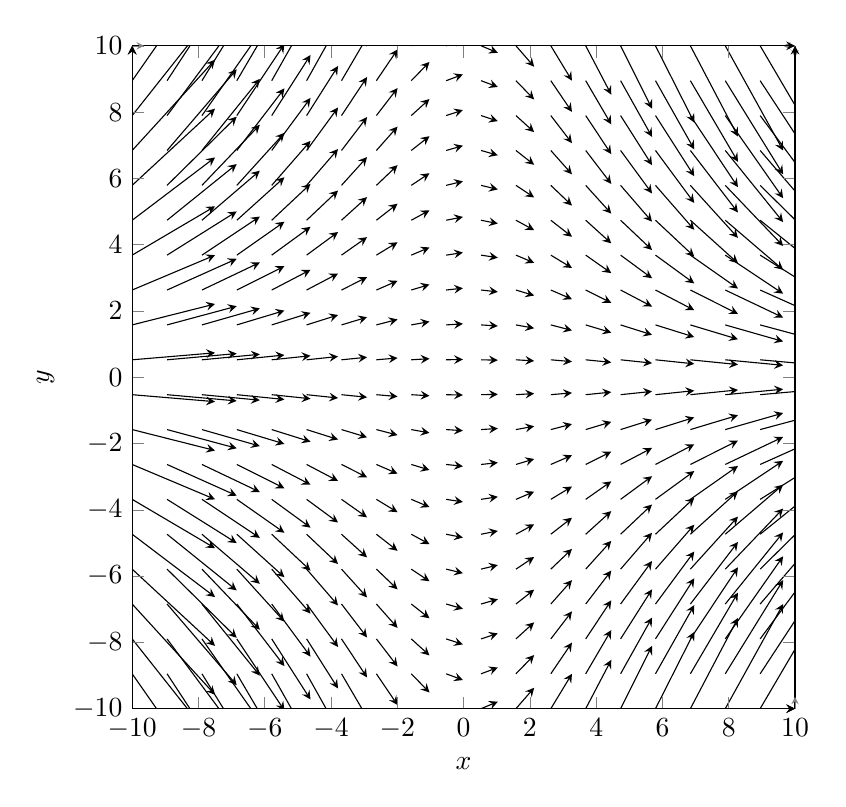
\begin{tikzpicture}
      \begin{axis}[
          width=10cm, % Width of the plot
          height=10cm, % Height of the plot
          xlabel={$x$},
          ylabel={$y$},
          xmin=-10, xmax=10, % x-axis range
          ymin=-10, ymax=10, % y-axis range
          axis equal image, % Keep the aspect ratio
          -stealth,
          view = {0}{90}
      ]
      % Define the constant d and B_0
      \pgfmathsetmacro{\d}{5} % Set d = 1 (example value)
      \pgfmathsetmacro{\Bzero}{1} % Set B_0 = 1 (example value)
      
      \addplot3[
          quiver={
              u={\Bzero*(1 + x^2/(\d^2))}, % x-component of the field
              v={\Bzero*(-2*x*y/(\d^2))},  % y-component of the field
              scale arrows=0.5, % Scale the arrow lengths
          },
          samples=20, % Number of samples for the grid
          domain=-10:10, % Domain for x
          y domain=-10:10 % Domain for y
      ] {0}; % 3D plot, z=0 since it's 2D
      \end{axis}
    \end{tikzpicture}
    \caption{Campo magnético inhomogéneo para $B_{0}=1$ y $d=5$.}
    \label{fig:field}
\end{figure}


\subsection{Describir las reglas de transformación Lorentz de la energía radiada por una carga}



\subsection{Se considera una función tensiorial $B_{\mu\nu}$ completamente antisymétrica (campo de Kalb-Ramond) que es potencial del campo \[H_{\lambda\mu\nu } = \partial_{\lambda} B_{\mu\nu } + \partial_{\nu} B_{\lambda\mu} + \partial_{\mu } B_{\nu \lambda }\].}



\begin{enumerate}
    \item[a)] Comprobar que $\partial_{\sigma} H^{* \sigma} = 0$, siendo $H^*$ el tensor dual de $H$.
    \item[b)] Dada la densidad lagrangiana 
    \[
    \mathcal{L} = - \frac{1}{6} H_{\lambda\mu\nu } H^{\lambda\mu\nu } - m^2 B_{\mu\nu} B^{\mu\nu},
    \]
    encontrar las ecuaciones de movimiento de $B_{\mu\nu}$.
    
    En primer lugar debemos poner el Lagrangiano en función de $B_{\mu \nu }$ como:
    \[\mathcal{L}= - \frac{1}{6} \left(\partial_{\lambda} B_{\mu\nu } + \partial_{\nu} B_{\lambda\mu} + \partial_{\mu } B_{\nu \lambda }\right)\left(\partial^{\lambda} B^{\mu\nu } + \partial^{\nu} B^{\lambda\mu} + \partial^{\mu } B^{\nu \lambda }\right)- m^2 B_{\mu\nu} B^{\mu\nu}\]
    \[\mathcal{L}= - \frac{1}{6} \left( \partial_{\lambda} B_{\mu\nu }\partial^{\lambda} B^{\mu\nu } + \partial_{\lambda} B_{\mu\nu }\partial^{\nu} B^{\lambda\mu} +\partial_{\lambda} B_{\mu\nu }\partial^{\mu } B^{\nu \lambda }+\partial_{\nu} B_{\lambda\mu}\partial^{\lambda} B^{\mu\nu } + \partial_{\nu} B_{\lambda\mu}\partial^{\nu} B^{\lambda\mu} +\partial_{\nu} B_{\lambda\mu}\partial^{\mu } B^{\nu \lambda }\right.\]
    \[\left. +\partial_{\mu } B_{\nu \lambda}\partial^{\lambda} B^{\mu\nu } + \partial_{\mu } B_{\nu \lambda}\partial^{\nu} B^{\lambda\mu} +\partial_{\mu } B_{\nu \lambda}\partial^{\mu } B^{\nu \lambda } \right)- m^2 B_{\mu\nu} B^{\mu\nu}\]

    \[\partial_{\mu }\frac{\partial\mathcal{L}}{\partial\partial_{\mu}B_{\mu \nu }}-\frac{\partial\mathcal{L}}{\partial B_{\mu \nu }}=0\]
    \item[c)] Se considera la siguiente transformación tipo-gauge: $B'_{\mu\nu} = B_{\mu\nu} + \partial_{\mu} \Psi_{\nu} - \partial_{\nu} \Psi_{\mu}$.
    Comprobar que el tensor $H$ es invariante gauge, analizar para qué valores de $m$ la lagrangiana $\mathcal{L}$ es invariante gauge.

    Primero escribimos la transformada del tensor H:
    \[H'_{\lambda\mu\nu } = \partial_{\lambda} B'_{\mu\nu } + \partial_{\nu} B'_{\lambda\mu} + \partial_{\mu } B'_{\nu \lambda }\]
    Y sustituimos la transformación Gauge para expresar $H'$ en función de $B$:
    \[H'_{\lambda\mu\nu } = \partial_{\lambda} \left(B_{\mu\nu } + \partial_{\mu} \Psi_{\nu} - \partial_{\nu } \Psi_{\mu} \right) + \partial_{\nu} \left(B_{\lambda\mu} + \partial_{\lambda  } \Psi_{\mu} - \partial_{\mu } \Psi_{\lambda} \right) + \partial_{\mu } \left(B_{\nu \lambda} + \partial_{\nu } \Psi_{\lambda} - \partial_{\lambda } \Psi_{\nu} \right) \]
    Reagrupamos términos 
    \[H'_{\lambda\mu\nu } =H_{\lambda\mu\nu } + \partial_{\lambda}\partial_{\mu} \Psi_{\nu} - \partial_{\lambda}\partial_{\nu} \Psi_{\mu} + \partial_{\nu}\partial_{\lambda  } \Psi_{\mu} - \partial_{\nu }\partial_{\mu} \Psi_{\lambda} + \partial_{\mu }\partial_{\nu} \Psi_{\lambda } - \partial_{\mu }\partial_{\lambda } \Psi_{\nu } \]
    Como el orden de las derivadas no es relevante, los terminos de $\Psi$ se cancelan y queda 
    \[H'_{\lambda\mu\nu } = H_{\lambda\mu\nu } \]
    Por lo tanto, el tensor $H$ es invariante gauge.

    Ahora, para analizar para qué valores de $m$ la lagrangiana $\mathcal{L}$ es invariante gauge, en donde el termino $- \frac{1}{6} H_{\lambda\mu\nu } H^{\lambda\mu\nu }$ es invariante por ser $H$ invariente, y quedaría solo comprobar el término $m^2 B_{\mu\nu} B^{\mu\nu}$, escribimos el Lagrangiano como:
    \[
    \mathcal{L}' = - \frac{1}{6} \underbrace{H_{\lambda\mu\nu } H^{\lambda\mu\nu }}_{\text{Invariante}} - m^2 B'_{\mu\nu} B'^{\mu\nu}
    \]
    Entonces 
    \[B'_{\mu\nu} B'^{\mu\nu}= \left(B_{\mu\nu} + \partial_{\mu} \Psi_{\nu} - \partial_{\nu} \Psi_{\mu}\right)\left(B^{\mu\nu} + \partial^{\mu} \Psi^{\nu} - \partial^{\nu} \Psi^{\mu}\right)\]
    \[B'_{\mu\nu} B'^{\mu\nu}=B_{\mu\nu} B^{\mu\nu} + B_{\mu\nu} \partial^{\mu} \Psi^{\nu} - B_{\mu\nu} \partial^{\nu} \Psi^{\mu} + \partial_{\mu} \Psi_{\nu} B^{\mu\nu} - \partial_{\nu} \Psi_{\mu} B^{\mu\nu} + \partial_{\mu} \Psi_{\nu} \partial^{\nu} \Psi^{\mu} - \partial_{\nu} \Psi_{\mu} \partial^{\mu} \Psi^{\nu} \]
\end{enumerate}


\end{document}

